\documentclass[letterpaper,10pt,a4paper]{article}
\usepackage{ulem}
\usepackage{url}

\usepackage{epsfig}
\usepackage{graphicx,color}% Include figure files
\usepackage{wrapfig,caption}
\usepackage{epstopdf}

\usepackage{fancyhdr,graphicx,epsfig,lastpage}
\usepackage{amsmath}
\usepackage{amssymb}

\usepackage{latexsym}
\usepackage[latin1,applemac]{inputenc}

%\usepackage{natbib}

\usepackage{booktabs}



\usepackage{mdwlist}
%\usepackage{enumitem}

%\usepackage[sort&compress,sectionbib]{natbib}
% \usepackage{german,isolatin1}
\usepackage{indentfirst}
%\usepackage{natbib}

\setlength{\parindent}{0in}
%\usepackage[superscript]{cite}

\usepackage{setspace} % Allows spacing of sections with \singlespacing and \doublespacing command

\oddsidemargin 0pt 
\evensidemargin 0pt 
\marginparwidth 68pt 
\marginparsep 10pt 
\topmargin 0pt 
\headheight 10pt 
\headsep 5pt

\voffset -40pt 
\footskip 35pt 
\textheight 23cm 
\textwidth 16.8cm 
\columnsep 10pt 
\columnseprule 0pt 
\sloppy 
%\frenchspacing

\linespread{1.27}

%\setlength{\parindent}{0pt} 
%\setlength{\parskip}{5pt plus 2pt minus 1pt}
%\renewcommand{\baselinestretch}{1.095} %{1.2} %{1.095}
%\clubpenalty=5000 \widowpenalty=5000
%\renewcommand{\footnoterule}{\vspace{0.5cm}%
%  \rule{2.5in}{0.4pt} \vspace{0.3cm}} \pagestyle{fancy}
%\renewcommand{\headrulewidth}{0.4pt} \lhead{Research Plan} \chead{}
%\rhead{\today} \renewcommand{\footrulewidth}{0.4pt} \lfoot{}
%\cfoot{\thepage /\pageref{LastPage}} \rfoot{}

%%%%%%%%%%%%%%%%%%%%%%%%%%%%%%%%%%%%%%%%%%%%%%%%%%%%%%%%%
% Main
%%%%%%%%%%%%%%%%%%%%%%%%%%%%%%%%%%%%%%%%%%%%%%%%%%%%%%%%%
\begin{document}
%\noindent
\begin{center}

  %\textbf{\Large Research Plan}\\[10mm]

%  \textbf{Title:}\\[5mm]
% \textbf{\Large Measuring Incentives for Attacks \& Security, }\\[4mm]
% \textbf{\Large and Managing Cyber Risk}\\ [10mm]

  %{\today}\\[85mm]

  %\textbf{PhD candidate:}\\
 % \textbf{\large Thomas Maillart}\\[10mm]

  %\textbf{Advisor:}\\
  %Prof. Dr. Didier Sornette\\
  %Chair of Entrepreneurial Risks\\
  %ETH Z\"urich (Swiss Federal Institute of Technology in Z\"urich)\\[5mm]

  % \textbf{Co-referee:}
  % \\[5mm]
  

\vspace{-0.5cm}
{\Large {\bf \textsc{Characterizing Contribution Strategies in Wikipedia with Bi-Partite Network Rankings\\}}}

\vspace{0.2cm}
{\large {\bf \textsc{Maximilian Klein, Thomas Maillart, John Chuang}}}
\vspace{0.15cm}
\end{center}

%Open source software has been one of the most successful incarnations of open innovation, providing considerable amount of software code as a public good for the development of reliable Internet and Web infrastructures, operating systems, and a broad range of applications.  Moreover, open source software (OSS) has inspired many initiatives beyond software development, such as Wikipedia  which combines (i) task self-selection and (ii) peer-review by participants.
\vspace{0.05cm}
%{\Large \bf Research Interests} \vspace{0.25cm}\\


%\clearpage
%\bibliography{../tmaillart.bib}
One of the very fundamental principles of peer-production in open collaboration projects is the ability for individuals to decide what tasks they want to 
take on \cite{benkler2002}. For instance, in Wikipedia editors touch varying numbers of articles, at different levels of development. The outstanding question is how individual contribution strategies are likely to influence the {\it investment} of each editor, the {\it quality} of articles \cite{wang}, and ultimately the quality of a project \cite{geiger2013}. One way to tackle the problem consists in considering a project -- here a category of Wikipedia articles -- as a bi-partite network of articles and their related editors \cite{jesus2009}. Assessing the value of the two types of components of such a network has previously been undertaken in the context of macro-economics (ranking countries by the type of products they export) by Hidalgo and Haussmann \cite{hidalgo2009}, and by Caldarelli et al. \cite{caldarelli2012network}. The investment of editors is assessed from the quantity and quality of articles they have edited. Conversely, the development of an article depends on the number and the investment of editors who have modified the article. The method is a two node-type version of the Google pageRank algorithm \cite{page1999pagerank} and can be compared to a random walker jumping between editors and articles. Walking is controlled by biased parameters $\alpha$ for the probability to jump to more developed articles, and $\beta$ for the probability to jump more invested editors (see Figure \ref{fig1}A). 
\begin{figure}[h]
\centering
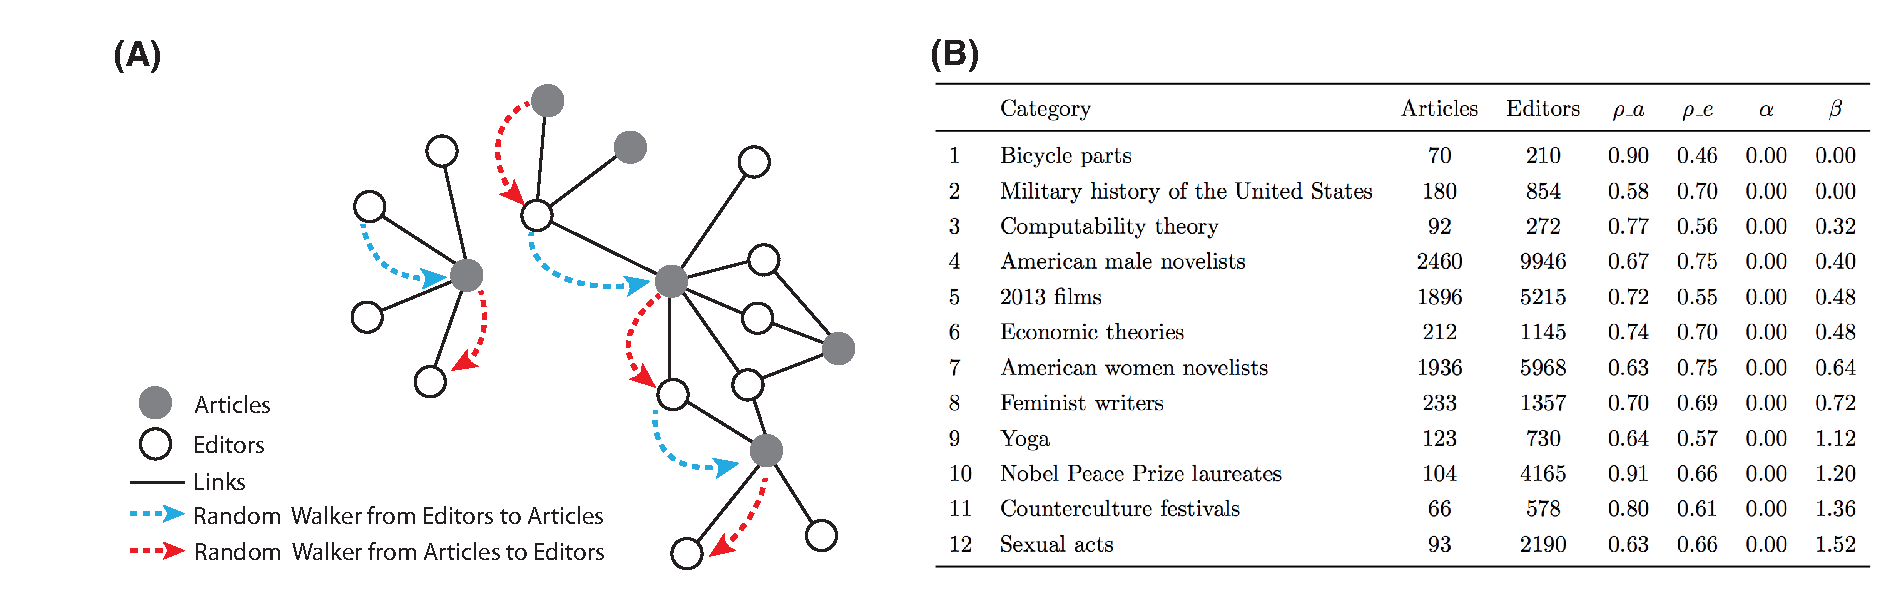
\includegraphics[width=0.8\columnwidth]{Figures/figure_abstract.eps}
\caption{{\bf (A)} Bi-partite network with Article and Editor nodes. Dashed arrows show how the random walker jumping between articles and editors with  probability controlled by the appropriately biased connectivity of the each node. {\bf (B)} Table shows the best rank-correlation $\rho_a$ and $\rho_e$ of the algorithm with the ground truth for each Wikipedia category, as well the value of the divestment bias $\beta$.}
\label{fig1}
\end{figure}

\begin{table}
\begin{tabular}{llll}
\toprule
                              Category & Editor divestment $\beta$  & $\rho_e$ & $\rho_a$ \\
\midrule
                         Bicycle parts &    0.00 &     0.46 &     0.90 \\
 Military history of the US &    0.00 &     0.70 &     0.58 \\
                  Computability theory &    0.32 &     0.56 &     0.77 \\
               American male novelists &    0.40 &     0.75 &     0.67 \\
                            2013 films &    0.48 &     0.55 &     0.72 \\
                     Economic theories &    0.48 &     0.70 &     0.74 \\
              American women novelists &    0.64 &     0.75 &     0.63 \\
                      Feminist writers &    0.72 &     0.69 &     0.70 \\
                                  Yoga &    1.12 &     0.57 &     0.64 \\
           Nobel Peace Prize laureates &    1.20 &     0.66 &     0.91 \\
              Counterculture festivals &    1.36 &     0.61 &     0.80 \\
                           Sexual acts &    1.52 &     0.66 &     0.63 \\
\bottomrule
\end{tabular}


\end{table}



The variables $\alpha$ and $\beta$ provide a direct measure of the nonlinear "importance" of the number of highly developed articles, and the nonlinear importance of highly invested editors, respectively. Both $\alpha$ and $\beta$ are optimized to maximize the rank correlations of editors ($0.46 < \rho_e < 0.75 $) and articles ($0.58 < \rho_a < 0.91$) between the algorithm and ground-truth metrics obtained by state-of-the-art quality metrics of editors \cite{geiger2013} and articles \cite{wang}, for 12 categories on Wikipedia. We find that the best value for $\alpha$ is $0$, while $0 \leqslant \beta \leqslant 1.52$ (c.f. Figure 1B). 

%We find that the importance of editor divestment is concave increasing as a function of the number of articles they have edited for categories with $\beta > 1$ and decreasing when $0 < \beta < 1$. For two categories ({\it bicycle parts} and {\it Military history of the US}), $\beta = 0$, so the investment of editors is actually a linear function of the number of articles they have edited. Regarding article correlations, the development is a linear function of the number of editors, and a function of the expertise of these editors, which in turn varies depending on the values of $\beta$. For $\beta = 0$, the expertise of editors has no influence, while for $\beta > 0$, the expertise provided by editors decreases as a function of the number of articles they have edited. 

Looking at \ref{fig1}B, we find telling extremes. The best editors in {\it Category:Military history of the US} - a category known for being very competitive -  are characterized by emphasizing investment (number of articles edited in the category). On the other end, the editors in {\it Category:Sexual acts} - a taboo subject where much editing could be considered perverse - are characterized by divesting in touching many articles in the category.




%\clearpage
\vspace{1cm}
\bibliographystyle{abbrv}
\bibliography{sigproc,tmaillart}  


\end{document}
